\documentclass{article}
\usepackage[T1]{fontenc}
\usepackage{lmodern}
\usepackage{graphicx}
\usepackage{amsmath,amssymb}
\usepackage[a4paper,margin=2cm]{geometry}
\usepackage[absolute,overlay]{textpos}
\setlength{\TPHorizModule}{1mm}
\setlength{\TPVertModule}{1mm}
\usepackage[indonesian]{babel}
\usepackage{hyperref}
\setlength{\emergencystretch}{2em}
% unit: Halaman 19

\begin{document}

% === Halaman 19 (python/native) ===

19

5. Chosen-ciphertext attack 

 Penyerang dapat memilih cipherteks tertentu dan mendekripsinya dengan 

oracle  yang bisa mendekripsi, dan menggunakan hasil dekripsi untuk 

memecahkan cipher atau menemukan kunci. 

      C1, P1 = Dk(C1), C2, P2 = Dk(P2), …,  Ci,  Pi = Dk(Ci)


 Deduksi: k  (yang mungkin diperlukan untuk mendekripsi pesan pada waktu 

yang akan datang).

% deskripsi: gambar native xref 151
\noindent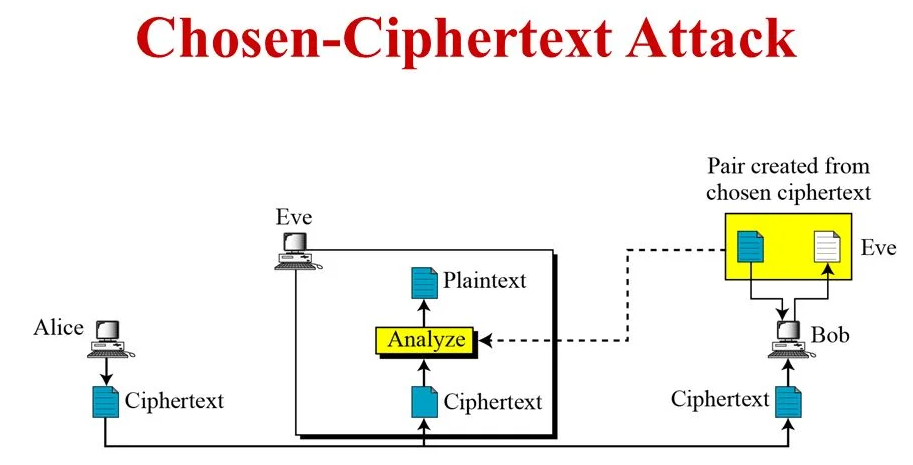
\includegraphics[width=0.85\textwidth]{../../images/python/page_019_img_01.png}

\end{document}
